\documentclass{beamer}
\usepackage{amsmath}
\usepackage{amsfonts}
\usepackage{graphicx}
\usepackage{tikz}
\usepackage{algorithm}
\usepackage{algorithmic}

\usetheme{Madrid}
\title{ADF \& TransApp: A Transformer-Based Framework for Appliance Detection}
\subtitle{Using Smart Meter Consumption Series}
\author{Adrien Petralia, Philippe Charpentier, Themis Palpanas}
\date{\today}

\begin{document}

\frame{\titlepage}

\begin{frame}{Overview}
\tableofcontents
\end{frame}

\section{Problem Formulation}

\begin{frame}{Problem Formulation}
\frametitle{Mathematical Setup}

\textbf{Time Series Definition:}
\begin{itemize}
    \item Electrical consumption time series: $X = (x_1, x_2, \ldots, x_T)$
    \item Each element $x_j \in \mathbb{R}^1_+$ represents consumption at timestamp $i_j$
    \item Very low frequency: sampled every 15-60 minutes
\end{itemize}

\vspace{0.5cm}

\textbf{Appliance Detection Problem:}
\begin{block}{Binary Classification Task}
Given: Collection of consumption time series $\mathcal{X} = \{X_1, X_2, \ldots, X_N\}$ of variable lengths

Goal: Predict presence/absence of appliance $a$ in time series $X_i$
\end{block}

\vspace{0.3cm}

\textbf{Challenge:} Long series (10k-20k points), variable lengths, low sampling frequency
\end{frame}

\begin{frame}{Problem Example}
\frametitle{Dummy Example}

\textbf{Input:} Smart meter data from household over 30 days
\begin{itemize}
    \item $X = (x_1, x_2, \ldots, x_{1440})$ where $T = 1440$ (30 days × 48 readings/day)
    \item $x_j$ = electricity consumption in kWh at 30-minute intervals
    \item Example values: $x_1 = 0.5$, $x_2 = 0.8$, $x_3 = 1.2$, ...
\end{itemize}

\vspace{0.3cm}

\textbf{Output:} Binary label for appliance presence
\begin{itemize}
    \item $y = 1$: Dishwasher present in household
    \item $y = 0$: No dishwasher in household
\end{itemize}

\vspace{0.3cm}

\textbf{Key Challenge:} At low sampling rates, individual appliance signatures are smoothed out and difficult to detect directly.
\end{frame}

\section{ADF Framework}

\begin{frame}{Appliance Detection Framework (ADF)}
\frametitle{Framework Overview}

\textbf{Core Idea:} Fragment long consumption series into manageable subsequences

\begin{algorithm}[H]
\caption{ADF Framework}
\begin{algorithmic}[1]
\STATE \textbf{Input:} Consumption series $X$ of length $l$
\STATE \textbf{Step 1:} Extract series from database
\STATE \textbf{Step 2:} Slice into $n = \lfloor l/w \rfloor$ subsequences of length $w$
\STATE \textbf{Step 3:} Add temporal encoding features
\STATE \textbf{Step 4:} Apply TransApp classifier to each subsequence
\STATE \textbf{Step 5:} Merge predictions using quantile-based aggregation
\STATE \textbf{Output:} Final binary prediction
\end{algorithmic}
\end{algorithm}

% Space for ADF architecture diagram
\vspace{0.5cm}
\begin{center}
\begin{figure}[h]
\centering
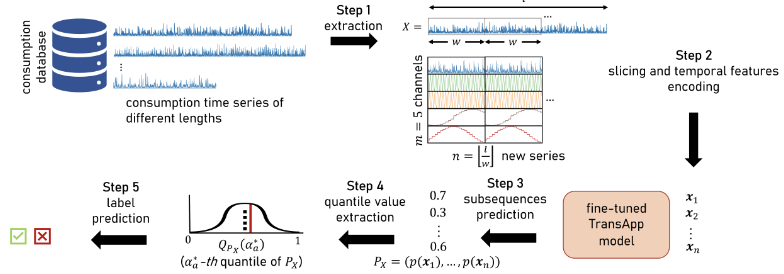
\includegraphics[width=0.5\textwidth]{adf.png}
\caption{ADF Framework Architecture}
\end{figure}
\end{center}

\end{frame}

\begin{frame}{ADF Step-by-Step Mathematics}
\frametitle{Detailed Mathematical Process}

\textbf{Step 2 - Subsequence Creation:}
\begin{align}
n &= \left\lfloor \frac{l}{w} \right\rfloor \\
\mathbf{x}_i &= X_{(i-1)w+1:(i-1)w+w} \quad \text{for } i = 1, 2, \ldots, n
\end{align}

\textbf{Step 3 - Temporal Encoding:}
\begin{align}
Te_{sin}(i_t) &= \sin\left(\frac{2\pi i_t}{p}\right) \\
Te_{cos}(i_t) &= \cos\left(\frac{2\pi i_t}{p}\right)
\end{align}
Where $p = 24$ for hours, $p = 7$ for days

\textbf{Result:} Each subsequence $\mathbf{x}_i$ becomes $\mathbf{x}_{w \times m}$ where $m$ is number of channels (consumption + temporal features)
\end{frame}

\begin{frame}{ADF Quantile-Based Aggregation}
\frametitle{Prediction Merging Strategy}

\textbf{Step 4 - Individual Predictions:}
\begin{itemize}
    \item TransApp predicts probability $p(\mathbf{x}_i)$ for each subsequence
    \item Results in probability vector: $P_X = (p(\mathbf{x}_1), p(\mathbf{x}_2), \ldots, p(\mathbf{x}_n))$
\end{itemize}

\vspace{0.3cm}

\textbf{Step 5 - Quantile Aggregation:}
\begin{align}
\alpha_a^* &= \arg\max_{\alpha \in \{0, 0.5, \ldots, 0.95, 1\}} S(y_{true}, y_{\alpha}^{pred}) \\
\text{Final Prediction} &= \text{round}(Q_{P_X}(\alpha_a^*))
\end{align}

Where $Q_{P_X}(\alpha_a^*)$ is the $\alpha_a^*$-th quantile of $P_X$

\vspace{0.3cm}

\textbf{Intuition:} Instead of simple majority voting, use quantile that maximizes validation performance
\end{frame}

\begin{frame}{ADF Example}
\frametitle{Concrete Example}

\textbf{Input Series:} $X$ with length $l = 2048$ points (21 days of 30-min data)

\textbf{Subsequence Creation:} Choose $w = 256$ (2.67 days)
\begin{itemize}
    \item $n = \lfloor 2048/256 \rfloor = 8$ subsequences
    \item $\mathbf{x}_1 = (x_1, x_2, \ldots, x_{256})$
    \item $\mathbf{x}_2 = (x_{257}, x_{258}, \ldots, x_{512})$
    \item ... and so on
\end{itemize}

\textbf{Temporal Encoding:} Each subsequence becomes $256 \times 5$ matrix
\begin{itemize}
    \item Channel 1: Original consumption values
    \item Channels 2-3: Hour encoding ($\sin, \cos$)
    \item Channels 4-5: Day encoding ($\sin, \cos$)
\end{itemize}

\textbf{Predictions:} $P_X = (0.2, 0.8, 0.9, 0.1, 0.7, 0.3, 0.85, 0.6)$
\textbf{Final Result:} If optimal $\alpha^* = 0.7$, then $Q_{P_X}(0.7) = 0.8 \rightarrow$ Label = 1
\end{frame}

\section{TransApp Architecture}

\begin{frame}{TransApp Architecture Overview}
\frametitle{Hybrid CNN-Transformer Design}

\textbf{Core Components:}
\begin{enumerate}
    \item \textbf{Embedding Block:} Convolutional feature extraction
    \item \textbf{Transformer Block:} Long-range dependency modeling
    \item \textbf{Task-specific Heads:} Classification or reconstruction
\end{enumerate}

\vspace{0.5cm}

\textbf{Input/Output Flow:}
\begin{align}
\mathbf{x}_{w \times m} \xrightarrow{\text{Embedding}} \mathbf{z}_{w \times d_{model}} \xrightarrow{\text{Transformer}} \mathbf{z}_{w \times d_{model}} \xrightarrow{\text{Head}} \text{Output}
\end{align}

Where $d_{model} = 96$ is the latent dimension

% Space for TransApp architecture diagram
\vspace{0.5cm}
\begin{center}

\begin{figure}[h]
\centering
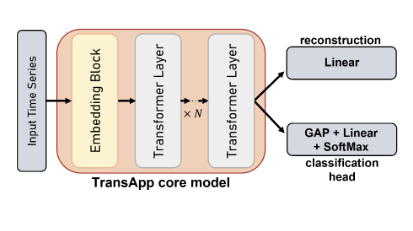
\includegraphics[width=0.6\textwidth]{trans-app.png}
\caption{TransApp Model Architecture}
\end{figure}

\end{center}

\end{frame}

\begin{frame}{Embedding Block Details}
\frametitle{Convolutional Feature Extraction}

\textbf{Architecture:} 4 stacked Residual Units (ResUnits)

\textbf{Each ResUnit contains:}
\begin{itemize}
    \item 1D Convolutional layer
    \item GeLU activation function
    \item BatchNormalization layer
    \item Residual connection
\end{itemize}

\vspace{0.3cm}

\textbf{Dilation Pattern:}
\begin{align}
\text{ResUnit}_i: \quad d = 2^i \quad \text{for } i = 1, 2, 3, 4
\end{align}

\textbf{Purpose:}
\begin{itemize}
    \item Exponentially increasing receptive fields
    \item Preserves time dimension (stride = 1)
    \item Provides inductive bias for local patterns
\end{itemize}

% Space for embedding block diagram
\vspace{0.3cm}


\end{frame}

\begin{frame}{Transformer Block Details}
\frametitle{Modified Attention Mechanism}

\textbf{Architecture:} $N$ stacked Transformer layers ($N = 3$ or $5$)

\textbf{Each layer contains:}
\begin{enumerate}
    \item Layer Normalization
    \item Multi-Head Diagonally Masked Self-Attention (DMSA)
    \item Layer Normalization
    \item Position-wise Feed-Forward Network (PFFN)
    \item Residual connections after DMSA and PFFN
\end{enumerate}

\vspace{0.3cm}

\textbf{Key Innovation - DMSA:}
\begin{itemize}
    \item Masks diagonal elements of attention matrix
    \item Attention scores: $A_{ii} = 0$ after softmax
    \item Emphasizes inter-token relationships
    \item Reduces overfitting on small datasets
\end{itemize}

\textbf{No Positional Encoding:} Temporal features already encoded in input
\end{frame}

\begin{frame}{TransApp Mathematical Flow}
\frametitle{Detailed Mathematical Operations}

\textbf{Input:} Subsequence $\mathbf{x}_{w \times m}$ where $w = 256$, $m = 5$

\textbf{Embedding Block:}
\begin{align}
\mathbf{h}_1 &= \text{ResUnit}_1(\mathbf{x}_{256 \times 5}) \rightarrow \mathbf{h}_1^{256 \times 32} \\
\mathbf{h}_2 &= \text{ResUnit}_2(\mathbf{h}_1) \rightarrow \mathbf{h}_2^{256 \times 64} \\
\mathbf{h}_3 &= \text{ResUnit}_3(\mathbf{h}_2) \rightarrow \mathbf{h}_3^{256 \times 96} \\
\mathbf{z} &= \text{ResUnit}_4(\mathbf{h}_3) \rightarrow \mathbf{z}^{256 \times 96}
\end{align}

\textbf{Transformer Block:}
\begin{align}
\mathbf{z}' &= \text{DMSA}(\text{LayerNorm}(\mathbf{z})) + \mathbf{z} \\
\mathbf{z}'' &= \text{PFFN}(\text{LayerNorm}(\mathbf{z}')) + \mathbf{z}'
\end{align}

\textbf{Output:} Final representation $\mathbf{z}_{256 \times 96}$
\end{frame}

\section{Two-Step Training Process}

\begin{frame}{Two-Step Training Overview}
\frametitle{Self-Supervised Pretraining + Supervised Fine-tuning}

\textbf{Motivation:}
\begin{itemize}
    \item Large amounts of unlabeled smart meter data available
    \item Limited labeled appliance data
    \item Transformer architectures benefit from pretraining
\end{itemize}

\vspace{0.5cm}

\textbf{Training Pipeline:}
\begin{enumerate}
    \item \textbf{Step 1:} Self-supervised pretraining on unlabeled consumption data
    \item \textbf{Step 2:} Supervised fine-tuning on labeled appliance data
\end{enumerate}

% Space for training process diagram
\vspace{0.5cm}


\end{frame}

\begin{frame}{Self-Supervised Pretraining}
\frametitle{Masked Reconstruction Task}

\textbf{Objective:} Learn consumption patterns without appliance labels

\textbf{Masking Process:}
\begin{itemize}
    \item Randomly mask 50\% of consumption channel
    \item Average mask segment length: $l_m = 24$ time steps (12 hours)
    \item Keep temporal encoding channels untouched
\end{itemize}

\vspace{0.3cm}

\textbf{Architecture:} TransApp + Reconstruction Head
\begin{align}
\mathbf{z}_{w \times d_{model}} \xrightarrow{\text{Linear Layer}} \hat{\mathbf{x}}_{w \times 1}
\end{align}

\textbf{Loss Function:} Mean Absolute Error on masked elements
\begin{align}
\mathcal{L}_{MAE} = \frac{1}{\#M} \sum_{i \in M} |\hat{x}_i - x_i|
\end{align}
Where $\#M$ is the number of masked elements

\end{frame}

\begin{frame}{Supervised Fine-tuning}
\frametitle{Appliance Classification Task}

\textbf{Objective:} Detect specific appliances using learned representations

\textbf{Architecture:} TransApp + Classification Head
\begin{align}
\mathbf{z}_{w \times d_{model}} \xrightarrow{\text{Global Avg Pool}} \mathbf{z}_{d_{model}} \xrightarrow{\text{Linear}} \text{logits}_2
\end{align}

\textbf{Training Details:}
\begin{itemize}
    \item Freeze or fine-tune pretrained weights
    \item Binary classification for each appliance type
    \item All subsequences inherit label from full series
\end{itemize}

\vspace{0.3cm}

\textbf{Loss Function:} Cross-entropy loss
\begin{align}
\mathcal{L}_{CE} = -\sum_{c=1}^{2} y_c \log(\sigma(\text{logits}_c))
\end{align}

\end{frame}

\begin{frame}{Why Two-Step Training Works}
\frametitle{Performance Benefits Analysis}

\textbf{Representation Learning Benefits:}
\begin{enumerate}
    \item \textbf{Pattern Recognition:} Learns general consumption patterns across households
    \item \textbf{Temporal Dependencies:} Captures daily/weekly consumption rhythms
    \item \textbf{Noise Robustness:} Develops robust features through reconstruction
    \item \textbf{Data Efficiency:} Leverages abundant unlabeled data
\end{enumerate}

\vspace{0.3cm}

\textbf{Experimental Evidence:}
\begin{itemize}
    \item TransAppPT (pretrained) vs TransApp (no pretraining)
    \item Average improvement: 1-2 percentage points in Macro F1-score
    \item Larger improvements with more pretraining data
    \item TransAppPT-l (pretrained on 200k series) achieves best results
\end{itemize}

\vspace{0.3cm}

\textbf{Scaling Effect:} Performance increases proportionally with pretraining data size
\end{frame}

\begin{frame}{Training Example}
\frametitle{Concrete Training Scenario}

\textbf{Pretraining Phase:}
\begin{itemize}
    \item Dataset: 200,000 unlabeled consumption series
    \item Input: Masked subsequences $\mathbf{x}_{256 \times 5}$
    \item Target: Reconstruct original consumption values
    \item Duration: 100 epochs
\end{itemize}

\vspace{0.3cm}

\textbf{Fine-tuning Phase:}
\begin{itemize}
    \item Dataset: 3,000 labeled series (dishwasher detection)
    \item Input: Complete subsequences $\mathbf{x}_{256 \times 5}$
    \item Target: Binary labels (dishwasher present/absent)
    \item Duration: 50 epochs
\end{itemize}

\vspace{0.3cm}

\textbf{Result:} 
\begin{itemize}
    \item TransApp (no pretraining): 0.564 Macro F1
    \item TransAppPT (pretrained): 0.594 Macro F1
    \item \textbf{Improvement: +3.0 percentage points}
\end{itemize}

\end{frame}

\section{Results and Conclusions}

\begin{frame}{Experimental Results}
\frametitle{Performance Summary}

\textbf{Datasets:}
\begin{itemize}
    \item CER: 3,470 Irish households, 9 appliance types
    \item EDF 1: 4,701 French households, 7 appliance types
    \item EDF 2: 200,000 unlabeled series for pretraining
\end{itemize}

\vspace{0.3cm}

\textbf{Key Findings:}
\begin{enumerate}
    \item ADF improves all baseline classifiers by 2-5 percentage points
    \item TransAppPT achieves best overall performance (rank 1-2)
    \item Pretraining on large unlabeled data provides significant gains
    \item Framework scales efficiently to long time series
\end{enumerate}

\vspace{0.3cm}

\textbf{Best Results:}
\begin{itemize}
    \item Water Heater detection: 0.855 Macro F1
    \item Electric Vehicle detection: 0.825 Macro F1
    \item Average across all appliances: 0.746 Macro F1
\end{itemize}

\end{frame}

\begin{frame}{Conclusions}
\frametitle{Key Contributions and Impact}

\textbf{Technical Contributions:}
\begin{enumerate}
    \item \textbf{ADF Framework:} Scalable approach for long, variable-length series
    \item \textbf{TransApp Architecture:} Hybrid CNN-Transformer with DMSA
    \item \textbf{Two-step Training:} Effective use of unlabeled data
    \item \textbf{Temporal Encoding:} Novel approach for time-aware features
\end{enumerate}

\vspace{0.3cm}

\textbf{Practical Impact:}
\begin{itemize}
    \item Enables real-world appliance detection for energy suppliers
    \item Supports personalized energy services and recommendations
    \item Contributes to energy transition goals
    \item Scalable to millions of smart meters
\end{itemize}

\vspace{0.3cm}

\textbf{Future Directions:}
\begin{itemize}
    \item Multi-appliance detection
    \item Real-time inference
    \item Cross-domain adaptation
\end{itemize}

\end{frame}

\end{document}